\chapter{Estado del arte} \label{ich:estado_arte}

Procedemos a realizar un estudio del estado del arte para el problema que buscamos resolver. En primer lugar, consultaremos el estado del arte para la tarea de \textit{retrieval } en reconocimiento facial invariante a la edad sobre el conjunto de datos \textit{CACD}, y en segundo lugar, para el conjunto de datos \textit{CACD}.

Como ya hemos comentado en \customref{isubsubs:fgnet_inconvenientes}, y motivados por el trabajo de \cite{informatica:best_fgnet_model}, nuestro enfoque va a ser el siguiente: realizar un entrenamiento sobre el conjunto de datos \textit{CACD}, y usar \textit{FG-Net} para validar nuestro modelo.

\section{Interés del área de estudio} \label{isec:interesareaestudio}

Empecemos viendo el interés de este área de estudio. Para ello podemos realizar una búsqueda en \textit{SCOPUS}, buscando trabajos sobre \textit{AIFR} en el campo de las ciencias de la computación. Esto produce los siguientes \textit{keywords}:

\begin{lstlisting}[caption=\textit{Keywords usados para la búsqueda en \textit{SCOPUS}}, label=code:scopus_search]
    TITLE-ABS-KEY ( age  AND invariant  AND face  AND recognition )  AND  ( LIMIT-TO ( SUBJAREA ,  "COMP" ) )
\end{lstlisting}

Con esto obtenemos la siguiente gráfica:

\begin{figure}[H]
    \centering
    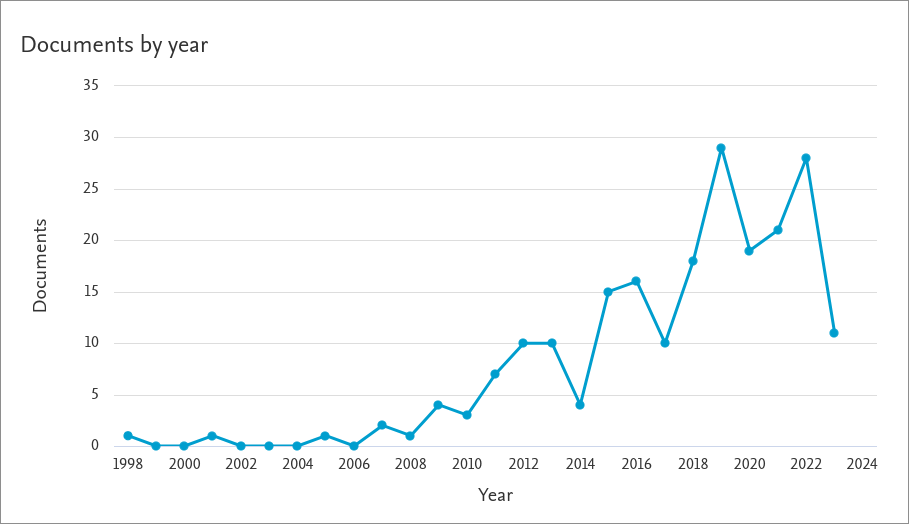
\includegraphics[width=0.6\textwidth]{informatica/scopus_search_histogram}
    \caption{Resultados de la búsqueda en \textit{SCOPUS} usando los \textit{keywords} \customref{code:scopus_search}}
\end{figure}

Vemos que, a partir de 2012 (momento que coincide con la aparición de \textit{AlexNet} y que da paso a la popularidad de redes convolucionales profundas en el campo de la imagen) este área de estudio gana bastante popularidad. Sin tener en cuenta el último año (pues, en el momento de la consulta, quedan unos meses para que acabe), no vemos que la tendencia siga al alza, pudiendo llegar a pensar que la popularidad de este campo se está estancando. Aunque habría que tener en cuenta condiciones externas, como la pandemia de \textit{COVID}, que podrían explicar la bajada notable en los años 2020 y 2021.

Sin embargo, estamos usando nuevas técnicas para computar \textit{triplet loss}. Dichas técnicas fueron introducidas en \cite{informatica:principal}. En dicho trabajo se intenta resolver una tarea de re-identificación, que difiere de nuestra tarea de \textit{retrieval} para reconocimiento facial invariante a la edad. Por lo tanto, búscamos trabajos que hayan aplicado \textit{triplet loss} en el campo del \textit{AIFR}. Aplicamos la siguiente búsqueda:

\begin{lstlisting}[caption=Keywords usandos para la búsqueda de trabajos que combinen \textit{AIFR} y \textit{triplet loss} en \textit{SCOPUS}, label=code:scopus_search_especifico]
    TITLE-ABS-KEY ( age AND invariant AND face AND recognition, AND triplet AND loss )  AND  ( LIMIT-TO ( SUBJAREA ,  "COMP" ) )
\end{lstlisting}

La búsqueda determinada por \customref{code:scopus_search_especifico} no produce ningún resultado. \textbf{No hay publicados ningún trabajo que aplique \textit{triplet loss} al campo del \textit{AIFR}}. Y esto, sin considerar que nuestro trabajo introduce nuevas técnicas que mejoran el uso del \textit{triplet loss} clásico, desarrollado en \customref{isec:triplet_loss}.

